\documentclass{memoir}
\usepackage{notestemplate}
\usetikzlibrary{matrix,arrows.meta}

%\logo{~/School-Work/Auxiliary-Files/resources/png/logo.png}
%\institute{Rice University}
%\faculty{Faculty of Whatever Sciences}
%\department{Department of Mathematics}
%\title{Class Notes}
%\subtitle{Based on MATH xxx}
%\author{\textit{Author}\\Gabriel \textsc{Gress}}
%\supervisor{Linus \textsc{Torvalds}}
%\context{Well, I was bored...}
%\date{\today}

%\makeindex

\begin{document}

% \maketitle

% Notes taken on 

The idea of a tensor product of modules \(M,N\) is to form another module in which we can take products \(mn\) of elements \(m \in M\) and \(n \in N\).

\begin{defn}[Ring Extension]
	Let \(R\leq S\). If \(\prescript{}{S}N\) is a left \(S\)-module, then \(N\) can also construct a left \(R\)-module since the elements of \(R\) act on \(N\) by assumption.\\

	More generally, if \(f:R\to S\) is a ring homomorphism from \(R\) into \(S\) with \(f(1_R) = 1_S\), then \(N\) can be considered as an \(R\)-module with \(rn = f(r)n\) for \(r \in R\) and \(n \in N\). We consider \(S\) a \textbf{ring extension of \(R\)} and the resulting \(R\)-module is said to be obtained from \(N\) by \textbf{restriction of scalars} from \(S\) to \(R\).
\end{defn}
One might wonder if the reverse can be done-- taking a ring \(R\) and attempting to extend the scalars to a larger ring. This cannot be done in general-- for example, one can check that \(\Z\) cannot be made into a \(\Q\)-module.\\

However, while \(\Z\) cannot be made into a \(\Q\)-module, it is contained in a \(\Q\)-module (\(\prescript{}{\Q}\Q\)). That is, there is an embedding of the \(\Z\)-module \(\prescript{}{\Z}\Z\) into the \(\Q\)-module \(\prescript{}{\Q}\Q\). This isn't always the case however-- to see this, consider the \(\Z\)-module \(\prescript{}{\Z}N\) where \(N\) is a finite abelian group. One can check that there are no nonzero homomorphisms into any \(\Q\)-module.\\

Our goal will be to construct a module which is the best candidate for which we can embed into.

\begin{defn}[Tensor Product of Modules]
	Let \(\prescript{}{R}N\) be a general \(R\)-module that we wish to embed into some \(S\)-modue. First we will try and define a product of the form \(sn\) for \(s \in S\), \(n \in N\).\\

	We start by considering the free \(\Z\)-module on the set \(S\times N\). This is the collection of all finite commuting sums of elements of the form \((s_i,n_i)\) with no relations imposed on \(sn\). Our \(S\)-module structure requires that we must satisfy the relations
	\begin{align*}
		r_1:& \quad(s_1+s_2)n = s_1n + s_2n \\
		r_2:& \quad s(n_1+n_2) = sn_1 + sn_2\\
		r_3:& \quad (sr)n = s(rn)
	\end{align*}
	for \(s_1,s_2,s \in S\), \(r \in R\), and \(n \in N\). We let \(H\leq N\) be the subgroup given by \(H := \langle r_1,r_2,r_3 \rangle \), that is, all elements of the form above, and consider \(N / H\). We denote this quotient group by \(S \otimes_R N\) and call it the \textbf{tensor module product of \(S\) and \(N\) over \(R\)}. We denote \(s \otimes n\) the coset containing \((s,n)\) in \(S \otimes_R N\) and so we have
	\begin{align*}
		(s_1+s_2) \otimes n = s_1\otimes n + s_2 \otimes n\\
		s \otimes (n_1+n_2) = s\otimes n_1 + s \otimes n_2\\
		sr \otimes n = s \otimes rn.
	\end{align*}
	The elements of \(S \otimes_R N\) are called \textbf{tensors of modules} and can be written as finite sums of \textbf{simple tensors of modules} of the form \(s \otimes n\) with \(s \in S, n \in N\).\\

	Now we give the tensor module product \(S \otimes_R N\) an \(S\)-module action by
	\begin{align*}
		s\left( \sum_{\textrm{finite}} s_i \otimes n_i \right) = \sum_{\textrm{finite}} (ss_i) \otimes n_i.
	\end{align*}
	We call this module \(\prescript{}{S}(S \otimes_R N)\) the \textbf{\(S\)-module obtained by extension of scalars from the \(R\)-module \(N\)}.
\end{defn}
The natural map \(\iota: N \to S \otimes_R N\) defined by \(n\mapsto 1 \otimes n\). Because \(1 \otimes rn = r(1 \otimes n)\), it follows that \(\iota\) is an \(R\)-module homomorphism from \(N\) to \(S \otimes_R N\). It is not injective in general, and so \(S \otimes_R N\) need not contain an isomorphic copy of \(N\).\\

Because the relatons imposed were the minimal relations necessary, one would expect that \(S \otimes_R N\) is the best possible \(S\)-module for a module homomorphism.

\begin{thm}[Universal Property for Tensor Modules]
	Let \(R\leq S\), let \(\prescript{}{R}N\) be a left \(R\)-module and let \(\iota: N \to S \otimes_R N\) be the \(R\)-module homomorphism defined by \(\iota(n) = 1 \otimes n\). Suppose that \(\prescript{}{S}L\) is an arbitrary left \(S\)-module and \(\varphi :N \to L\) is an \(R\)-module homomorphism from \(N\) to \(L\). Then there is a unique \(S\)-module homomorphism \(\Phi :S \otimes_R N \to L\) such that \(\varphi = \Phi \circ \iota \) and the diagram commutes:
\begin{center}
			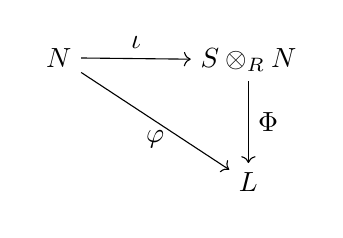
\begin{tikzpicture}
  \matrix (m)
    [
      matrix of math nodes,
      row sep    = 3em,
      column sep = 4em
    ]
    {
	    N & S \otimes_R N \\
	     & L            \\
    };
  \path
  (m-1-2) edge [->] node [right] {\(\Phi \)} (m-2-2)
    (m-1-1) edge [->] node [above] {\(\iota\)} (m-1-2)
      (m-1-1) edge [->] node [below] {$\varphi$} (m-2-2);
\end{tikzpicture}
\end{center}
Conversely, if \(\Phi :S \otimes_R N \to L\) is an \(S\)-module homomorphism then \(\varphi  = \Phi \circ \iota\) is an \(R\)-module homomorphism from \(N\) to \(L\).
\end{thm}

\begin{cor}
	Let \(\iota:N \to S \otimes_R N\) be the \(R\)-module homomorphism from the universal property of free modules. Then \(N / \textrm{Ker}\iota\) is the unique largest quotient of \(N\) that can be embedded in any \(S\)-module.\\

	In particular, \(N\) can be embedded as an \(R\)-submodule of some left \(S\)-module if and only if \(\iota\) is injective.
\end{cor}

\begin{exmp}
	
\end{exmp}


\subsection{General Tensor Product}
\label{sub:general_tensor_product}

Notice that forming \(S\otimes_R N\) as an abelian group only required \(S_R\) to be a right \(R\)-module and \(\prescript{}{R}N\) a left \(R\)-module. We can construct an abelian group \(M \otimes_R N\) for any right \(R\)-module \(M_R\) and any left \(R\)-module \(\prescript{}{R}N\).\\

The \(S\)-module structure on \(\prescript{}{S}{(S \otimes_R N)}\) required only a left \(S\)-module structure on \(\prescript{}{S}S\) and the compatibility relation
\begin{align*}
	s'(^2) = (s's)r.
\end{align*}

\begin{defn}[Tensor]
	Let \(\prescript{}{R}N\) be a left \(R\)-module and \(M_R\) a right \(R\)-module. We obtain an abelian group by quotient of the free \(\Z\)-module on \(M\times N\) by the subgroup \(H = \langle r_1,r_2,r_3 \rangle \), where
	\begin{align*}
		r_1:& \quad (m_1+m_2,n) = (m_1,n) + (m_2,n)\\
		r_2:& \quad (m, n_1+n_2) = (m,n_1) + (m,n_2)\\
		r_3:& \quad (mr,n) = (m,rn)
	\end{align*}
	for \(m,m_1,m_2 \in M\), \(n,n_1,n_2 \in N\), and \(r \in R\). We denote this by
	\begin{align*}
		M \otimes_R N := \prescript{}{\Z}(M \times N) / \langle r_1,r_2,r_3 \rangle 
	\end{align*}
	and call it the \textbf{tensor product of \(M\) and \(N\) over \(R\)}. The elements of \(M \otimes_R N\) are called \textbf{tensors}, and the coset \(m \otimes n \in M \otimes_R N\) is called a \textbf{simple tensor}. Every tensor can be written (non-uniquely) as a finite sum of simple tensors.
\end{defn}
Keep in mind that \(m \otimes n\) are cosets and not elements directly-- so caution must be used when defining maps on tensor products. That is, one needs to check that a map is well-defined on the entirety of a coset.\\

Furthermore, caution must be exercised when comparing tensor products. For example, if \(M \leq M'\), we can have \(m \otimes n = 0\) in \(M' \otimes_R N\) but \(m \otimes n \neq 0\) in \(M \otimes_R N\). This essentially captures the notion that when more elements are included, the cosets will change. Hence there is no reason to expect \(M \otimes_R N \leq M' \otimes_R N\).

\begin{defn}
	Let \(M_R\) be a right \(R\)-module, \(\prescript{}{R}N\) a left \(R\)-module, and \(L\) an abelian group. A map \(\varphi :M\times N \to L\) is called \textbf{\(R\)-balanced} or \textbf{middle linear with respect to \(R\)} if
	\begin{align*}
		\varphi (m_1+m_2,n) &= \varphi(m_1,n) + \varphi (m_2,n)\\
		\varphi (m,n_1+n_2) &= \varphi (m,n_1) + \varphi (m,n_2)\\
		\varphi (m,rn) &= \varphi (mr,n)
	\end{align*}
	for all \(m,m_1,m_2 \in M\), \(n,n_1,n_2 \in N\) and \(r \in R\).
\end{defn}
We can define a map \(\iota:M\times N \to M \otimes_R N\) with \(\iota(m,n) = m \otimes n\). This map is not a group homomorphism but it is in fact \(R\)-balanced.

\begin{thm}[Universal Property of Tensor Products]
	Let \(R\) be a ring, \(M_R\) a right \(R\)-module, and \(\prescript{}{R}N\) a left \(R\)-module. Let \(M \otimes_R N\) be the tensor product of \(M\) and \(N\) over \(R\) and let \(\iota: M \times N \to M \otimes_R N\) be the \(R\)-balanced map defined by \(\iota(m,n) = m \otimes n\). Then for any group homomorphism \(\Phi :M \otimes_R N \to L\) to an abelian group \(L\), the composite map
	\begin{align*}
		\varphi = \Phi \circ \iota
	\end{align*}
	is an \(R\)-balanced map from \(M \times N \to L\). Conversely, if \(L\) is an abelian group and \(\varphi :M \times N \to L\) is any \(R\)-balanced map, then there is a unique group homomorphism \(\Phi: M \otimes_R N \to L\) such that \(\varphi  = \Phi \circ \iota\).\\

	In other words, there is a correspondence between \(\varphi \) and \(\Phi \) by the commutative diagram:
\begin{center}
			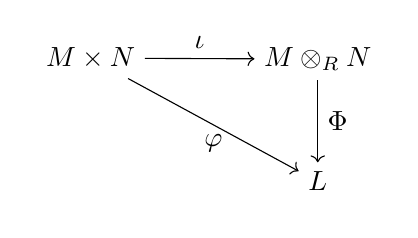
\begin{tikzpicture}
  \matrix (m)
    [
      matrix of math nodes,
      row sep    = 3em,
      column sep = 4em
    ]
    {
	    M \times N & M \otimes_R N \\
	     & L            \\
    };
  \path
  (m-1-2) edge [->] node [right] {\(\Phi \)} (m-2-2)
    (m-1-1) edge [->] node [above] {\(\iota\)} (m-1-2)
      (m-1-1) edge [->] node [below] {$\varphi$} (m-2-2);
\end{tikzpicture}
\end{center}
and this correspondence establishes a bijection between \(R\)-balanced maps and group homomorphisms, by the bijection between \(\varphi \) and \(\Phi \).
\end{thm}

\begin{cor}
	Suppose \(D\) is an abelian group and \(\iota':M \times N \to D\) is an \(R\)-balanced map such that
	\begin{itemize}
		\item \(D = \langle \textrm{Im}(\iota')\rangle \) 
		\item every \(R\)-balanced map defined on \(M\times N\) factors through \(\iota'\)
	\end{itemize}
	Then there is an isomorphism \(f: M \otimes_R N \cong D\) of abelian groups with \(\iota' = f \circ \iota\)
\end{cor}

Now we'd like to give this abelian group a module structure. We simply need to impose a compatibility structure on \(M\) to obtain this.

\begin{defn}
	Let \(R,S\) be rings. An abelian group \(M\) induces a \textbf{\((S,R)\)-bimodule} if \(M\) forms a left \(S\)-module, a right \(R\)-module, and \(s(mr) = (sm)r\) for all \(s \in S, r \in R, m \in M\).
\end{defn}

\begin{exmp}
	Let \(R\) be a commutative ring. A left \(R\)-module \(\prescript{}{R}M\) can always be given the structure of a right \(R\)-module by simply defining \(mr = rm\), and hence \(M\) becomes a \((R,R)\)-bimodule. We call this the \textbf{standard} \(R\)-module structure on \(M\).
\end{exmp}
Notice that if \(N\) has a left \(R\)-module structure and \(M\) a \((S,R)\)-bimodule structure, then we have once again
\begin{align*}
	s \left( \sum_{\textrm{finite}} m_i \otimes n_i \right) = \sum_{\textrm{finite}} (sm_i) \otimes n_i
\end{align*}
and hence there is a well-defined action of \(S\) so that \(M \otimes_R N\) can be considered a left \(S\)-module. It follows that for fixed \(s\), \((m,n)\mapsto sm \otimes n\) is an \(R\)-balanced map, and hence there is a well-defined group homomorphism \(\lambda_s:M\otimes_R N \to M \otimes_R N\) that satisfies \(\lambda_s(m \otimes n) = sm \otimes n\).\\

A special case we might encounter is when \(M,N\) are left modules over a commutative ring \(R\), and \(S = R\). Then the standard \(R\)-module structure on \(M\) gives \(M\) the structure of an \((R,R)\)-bimodule and hence \(M \otimes_R N\) always has the structure of a left \(R\)-module.

\begin{defn}
	Let \(R\) be a commutative ring and let \(M,N,L\) be left \(R\)-modules. The map \(\varphi : M \times N \to L\) is called \textbf{\(R\)-bilinear} if it is \(R\)-linear in every factor:
	\begin{align*}
		\varphi (r_1m_1+r_2m_2,n) &= r_1 \varphi (m_1,n) + r_2 \varphi (m_2,n)\\
		\varphi (m,r_1n_1 + r_2n_2) = r_1 \varphi (m,n_1) + r_2 \varphi (m,n_2)
	\end{align*}
	for all \(m, m_1, m_2 \in M\), \(n,n_1,n_2 \in N\), and \(r_1,r_2 \in R\).
\end{defn}

\begin{cor}
	Suppose \(R\) is a commutative ring, and \(M,N\) two left \(R\)-modules. Let \(M \otimes_R N\) be the tensor product of \(M\) and \(N\) over \(R\), where \(M\) is given the standard \(R\)-module structure. Then \(M \otimes_R N\) is a left \(R\)-module with
	\begin{align*}
		r(m \otimes n) = (rm) \otimes n = (mr) \otimes n = m \otimes (rn)
	\end{align*}
	and the map \(\iota:M \times N \to M \otimes_R N\) with \(\iota(m,n) = m \otimes n\) is an \(R\)-bilinear map. If \(L\) is any left \(R\)-module then there is a bijection between \(R\)-bilinear maps and \(R\)-module homomorphisms induced by the bijection between \(\varphi: M\times N \to L \) and \(\Phi: M \otimes_R N \to L \) via the commutative diagram:
\begin{center}
			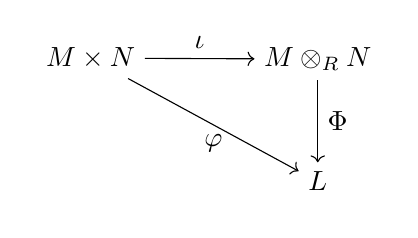
\begin{tikzpicture}
  \matrix (m)
    [
      matrix of math nodes,
      row sep    = 3em,
      column sep = 4em
    ]
    {
	    M \times N & M \otimes_R N \\
	     & L            \\
    };
  \path
  (m-1-2) edge [->] node [right] {\(\Phi \)} (m-2-2)
    (m-1-1) edge [->] node [above] {\(\iota\)} (m-1-2)
      (m-1-1) edge [->] node [below] {$\varphi$} (m-2-2);
\end{tikzpicture}
\end{center}
\end{cor}

\begin{exmp}
		
\end{exmp}

\begin{thm}[Tensor Product of Homomorphisms]
	Let \(M, M'\) be right \(R\)-modules, let \(N,N'\) be left \(R\)-modules. Suppose \(\varphi :M \to M'\) and \(\psi : N \to N'\) are \(R\)-module homomorphisms. Then there is a unique group homomorphism denoted by \(\varphi  \otimes \psi \) given by
	\begin{align*}
		\varphi \otimes \psi : M \otimes_R N \to M' \otimes_R N'\\
		(\varphi \otimes \psi )(m \otimes n) = \varphi (m) \otimes \psi (n)
	\end{align*}
	for all \(m \in M\) and \(n \in N\).\\

	If \(M,M'\) are \((S,R)\)-bimodules for some ring \(S\), and \(\varphi \) is also an \(S\)-module homomorphism, then \(\varphi \otimes \psi \) is a homomorphism of left \(S\)-modules. Hence if \(R\) is commutative then \(\varphi \otimes \psi \) is always an \(R\)-module homomorphism for the standard \(R\)-module structures.
\end{thm}
Notice that the uniqueness conditions tells us that if \(\lambda :M' \to M''\) and \(\mu : N' \to N''\) are \(R\)-module homomorphisms, then
\begin{align*}
	(\lambda \otimes u ) \circ (\varphi  \otimes \psi ) = (\lambda \circ \varphi ) \otimes (\mu  \otimes \psi ).
\end{align*}
In fact, we can use this idea to extend the tensor product into an \(n\)-fold tensor product.

\begin{thm}
	Suppose \(M\) is a right \(R\)-module, \(N\) is an \((R,T)\)-bimodule, and \(L\) is a left \(T\)-module. Then there is a unique isomorphism
	\begin{align*}
		(M \otimes_R N) \otimes_T L \cong M \otimes_R (N \otimes_T L)
	\end{align*}
	of abelian groups such that
	\begin{align*}
		(m \otimes_R n) \otimes l \mapsto m \otimes_R(n \otimes_R l).
	\end{align*}
	If \(M\) is an \((S,R)\)-bimodule, then this is an isomorphism of \(S\)-modules.
\end{thm}

\begin{cor}
	Let \(R\) be a commutative ring and \(M,N,L\) form left \(R\)-modules. Then
	\begin{align*}
		(M \otimes_R N) \otimes_R L \cong M \otimes_R(N \otimes_R L)
	\end{align*}
\end{cor}
Of course, it will be useful to use the natural extension of a bilinear map.

\begin{defn}
	Let \(R\) be a commutative ring and  let \(M_1,M_2,\ldots,M_n\) and \(L\) form \(R\)-modules with the standard \(R\)-module structures. A map \(\varphi : M_1 \times  \ldots \times M_n \to L\) is called \textbf{\(n\)-multilinear over \(R\)} if it is an \(R\)-module homomorphism in each component:
	\begin{align*}
		\varphi (m_1,\ldots,m_{i-1},rm_i + r'm'_i, m_{i+1},\ldots,m_n) = r \varphi(m_1,\ldots,m_i,\ldots,m_n) + r' \varphi (m_1,\ldots,m_i', \ldots, m_n)
	\end{align*}
\end{defn}
Hence we can define an \(n\)-fold tensor product by iterating the tensor product of pairs of modules.

\begin{cor}
	Let \(R\) be a commutative ring and let \(M_1,\ldots,M_n,L\) be \(R\)-modules. Let \(M_1 \otimes_R M_{2} \otimes_R \ldots \otimes_R M_n\) be the sequence of tensor products of pairs of these modules and let
	\begin{align*}
		\iota:M_1\times \ldots \times M_n \to M_1 \otimes_R \ldots \otimes_R M_n\\
		\iota(m_1,\ldots,m_n) = m_1 \otimes_R \ldots \otimes_R m_n.
	\end{align*}
	Then for every \(R\)-module homomorphism \(\Phi : M_1 \otimes_R \ldots \otimes_R M_n \to L\) the map \(\varphi = \Phi \circ \iota\) is \(n\)-multilinear from \(M_1\times \ldots\times M_n\to L\).\\

	If \(\varphi :M_1\times \ldots\times M_n \to L\) is an \(n\)-multilinear map then there is a unique \(R\)-module homomorphism \(\Phi :M_1 \otimes_R \ldots \otimes_R M_n \to L\) such that \(\varphi  = \Phi \circ \iota\). This bijection induces a bijection between \(n\)-multilinear maps and \(R\)-module homomorphisms for which the following diagram commutes:
\begin{center}
			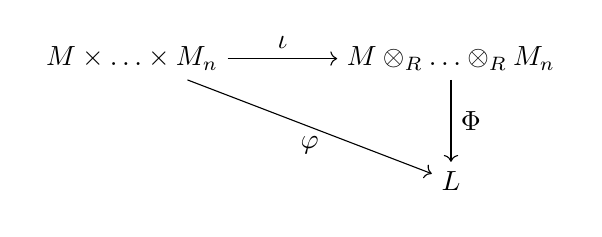
\begin{tikzpicture}
  \matrix (m)
    [
      matrix of math nodes,
      row sep    = 3em,
      column sep = 4em
    ]
    {
	    M \times \ldots \times M_n & M \otimes_R \ldots \otimes_R M_n \\
	     & L            \\
    };
  \path
  (m-1-2) edge [->] node [right] {\(\Phi \)} (m-2-2)
    (m-1-1) edge [->] node [above] {\(\iota\)} (m-1-2)
      (m-1-1) edge [->] node [below] {$\varphi$} (m-2-2);
\end{tikzpicture}
\end{center}
\end{cor}

We once again have a containment condition.

\begin{thm}[Tensor Products of Direct Sums]
	Let \(M, M'\) be right \(R\)-modules and let \(N, N'\) be left \(R\)-modules. Then there are unique group isomorphisms
	\begin{align*}
		(M \oplus M') \otimes_R N \cong (M \otimes_R N) \oplus (M' \otimes_R N)\\
		M \otimes_R (N \oplus N') \cong (M \otimes_R N) \oplus (M \otimes_R N')\\
		(m,m') \otimes n \mapsto (m \otimes n, m' \otimes n)\\
		m \otimes(n,n') \mapsto (m \otimes n, m \otimes n').
	\end{align*}
	If \(M,M'\) are also \((S,R)\)-bimodules, then these are isomorphisms of left \(S\)-modules. In particular, if \(R\) is commutative, these are isomorphisms of \(R\)-modules.
\end{thm}
Of course, this theorem extends inductively to any finite direct sum of \(R\)-modules (in fact any arbitrary direct sums). In essense, tensor products commute with direct sums.

\begin{cor}
	The module obtained from the free \(R\)-module \(N \cong \prescript{}{R}R^{n}\) by extension of scalars from \(R\) to \(S\) is the free \(S\)-module \(\prescript{}{S}S^{n}\):
	\begin{align*}
		S \otimes_R R^{n} \cong S^{n}
	\end{align*}
as left \(S\)-modules.
\end{cor}

\begin{cor}
	Let \(R\) be a commutative ring and let \(M \cong R^{s}\), \(N \cong R^{t}\) form free \(R\)-modules with bases \(m_1,\ldots,m_s\) and \(n_1,\ldots,n_t\) respectively.  Then \(M \otimes_R N\) forms a free \(R\)-module of rank \(st\) with basis \(m_i \otimes n_j\), \(1\leq i\leq s\) and \(1\leq j\leq t\), so that:
	\begin{align*}
		R^{s} \otimes_R R^{t} \cong R^{st}.
	\end{align*}
\end{cor}

\begin{rmrk}
	The tensor product of two free modules of arbitrary rank over a commutative ring is free.
\end{rmrk}

\begin{prop}
	Suppose \(R\) is a commutative ring and \(M,N\) form left \(R\)-modules via the standard \(R\)-module structures. Then there is a unique \(R\)-module isomorphism
	\begin{align*}
		M \otimes_R N \cong N \otimes_R M\\
		m \otimes n \mapsto n \otimes m
	\end{align*}
\end{prop}
One might think that if \(M=N\), the above conditions are not necessary, but in fact it is not the case. Some tensors do have the property that \(a \otimes b = b \otimes a\) for \(a,b \in M\), which we refer to as symmetric tensors, to be studied later.

\begin{prop}
	Let \(R\) be a commutative ring and let \(A,B\) be \(R\)-algebras. Then the multiplication
	\begin{align*}
		(a \otimes b) (a' \otimes b') = a a' \otimes b b'
	\end{align*} is well-defined and makes \(A\otimes_R B\) into an \(R\)-algebra.
\end{prop}

\begin{exmp}
	
\end{exmp}

% \printindex
\end{document}
